\section{Thiết kế cơ sở dữ liệu}

% TODO: add specific database design for the system

Dựa theo những yêu cầu và thiết kế, cơ sở dữ liệu của hệ thống được thiết kế
như Hình 3.19. Hệ thống sử dụng CSDL PostgreSQL được host trên nền tảng Supabase. Với cụ thể thông tin các bảng như sau: 
\subsection{Các bảng dữ liệu chính}
\begin{itemize}
    \item \textbf{image}: Lưu trữ thông tin về các hình ảnh được người dùng tải lên. Bảng này chứa các trường quan trọng như "image\_bucket\_id" và "image\_name" (liên kết đến đối tượng lưu trữ trong storage), "uploader\_id" (người tải lên), "image\_features" (vector đặc trưng của ảnh dùng cho tìm kiếm), "labels" (nhãn được gắn tự động), thông tin vị trí (longitude, latitude) và trạng thái nhận dạng khuôn mặt.
    
    \item \textbf{person}: Lưu trữ thông tin về các khuôn mặt được phát hiện trong ảnh. Mỗi bản ghi chứa "embedding" (vector đặc trưng khuôn mặt), "coordinate" (vị trí của khuôn mặt trong ảnh), "image\_id" (ảnh chứa khuôn mặt), "user\_id" (chủ sở hữu) và "cluster\_id" (nhóm khuôn mặt tương tự).
    
    \item \textbf{cluster\_mapping}: Quản lý các nhóm khuôn mặt tương tự nhau, với các trường chính là "name" (tên nhóm, có thể là tên người) và "centroid" (vector đại diện cho nhóm khuôn mặt).
    
    \item \textbf{album}: Lưu trữ thông tin về các album do người dùng tạo ra, với các trường quan trọng là "owner\_id" (người tạo) và "name" (tên album).
    
    \item \textbf{album\_image}: Bảng liên kết giữa album và hình ảnh, cho biết hình ảnh nào thuộc album nào.
    
    \item \textbf{search\_history}: Lưu trữ lịch sử tìm kiếm của người dùng, bao gồm "content" (nội dung tìm kiếm), "user\_id" (người tìm kiếm). Ngoài ra trường "text\_features" (vector đặc trưng của nội dung tìm kiếm) được sử dụng để tìm kiếm hình ảnh theo câu hỏi truy vấn của người dùng. 
    
    \item \textbf{video\_render}: Quản lý thông tin về các video slideshow, bao gồm "request\_user\_id" (người yêu cầu tạo video), "status" (trạng thái render video), "progress" (tiến độ hoàn thành), "schema" (kịch bản và option video) và "thumbnail\_url" (link ảnh đại diện video)
    
    \item \textbf{video\_chunk}: Lưu trữ thông tin về các phân đoạn của video được tạo ra theo chuẩn HLS, liên kết với video\_id và có thông tin về tên và vị trí lưu trữ của từng chunk.
    
    \item \textbf{video\_image}: Bảng liên kết giữa video và các hình ảnh được sử dụng trong video đó.
\end{itemize}

\subsection{Tích hợp với các bảng hệ thống của Supabase}

Ngoài các bảng được định nghĩa trong schema public, hệ thống còn sử dụng hai bảng đặc biệt có sẵn của Supabase:

\begin{itemize}
    \item \textbf{auth.user}: Quản lý thông tin xác thực và tài khoản người dùng, được cung cấp bởi hệ thống xác thực của Supabase. Bảng này lưu trữ thông tin như email, mật khẩu (đã được mã hóa), thời gian đăng ký và đăng nhập cuối cùng. Nhiều bảng trong hệ thống tham chiếu đến bảng này dưới hình thức khóa ngoại, để khi người dùng xóa tài khoản, các thông tin không còn cần thiết trong các bảng khác cũng sẽ được xóa theo.
    
    \item \textbf{storage.objects}: Quản lý các đối tượng lưu trữ (tệp) trong hệ thống lưu trữ của Supabase. Hệ thống sử dụng bảng này để lưu trữ ảnh trong thư viện, ảnh đại diện và các chunk video recap của người dùng.
\end{itemize}

Thiết kế cơ sở dữ liệu này cho phép hệ thống Smart Gallery lưu trữ và quản lý hiệu quả các dữ liệu liên quan đến hình ảnh, khuôn mặt, album, tìm kiếm và video, đồng thời tận dụng các tính năng xác thực và lưu trữ có sẵn của Supabase.

\subsection{Triggers và Functions tự động}

Ngoài các bảng dữ liệu chính, hệ thống còn sử dụng 2 tính năng của cơ sở dữ liệu PostgreSQL là triggers và functions để tự động hóa một số quy trình trong cơ sở dữ liệu. Cụ thể:
\begin{itemize}
    \item \textbf{trigger\_image\_face\_detection}: 1 Trigger được kích hoạt khi có 1 ảnh mới được chèn vào bảng "images". Tự động thông báo cho server để xử lý và phát hiện khuôn mặt trong bức ảnh.
    
    % \newpage
    % \lstinputlisting[
    %     language=SQL,
    %     caption=Trigger thông báo cho server xử lý ảnh,
    %     inputencoding=utf8,
    %     numberstyle=\small\color{gray},
    % ]{snipet/sql/search_similar_images.sql}
    
    \item \textbf{search\_similar\_images}: 1 Function được sử dụng để tìm kiếm các hình ảnh tương tự trong cơ sở dữ liệu dựa trên vector đặc trưng của hình ảnh. Hàm này sử dụng phương pháp tìm kiếm cosine similarity để tìm ra các hình ảnh có vector tương tự nhất với vector đầu vào. Hàm này được gọi từ server khi người dùng thực hiện tìm kiếm hình ảnh. 
    
    % \lstinputlisting[
    %     language=SQL,
    %     caption=Function tìm kiếm hình ảnh tương tự,
    %     inputencoding=utf8,
    %     numberstyle=\small\color{gray},
    % ]{snipet/sql/notify_face_detection.sql}
\end{itemize}

\begin{figure}[H]
    \centering  
    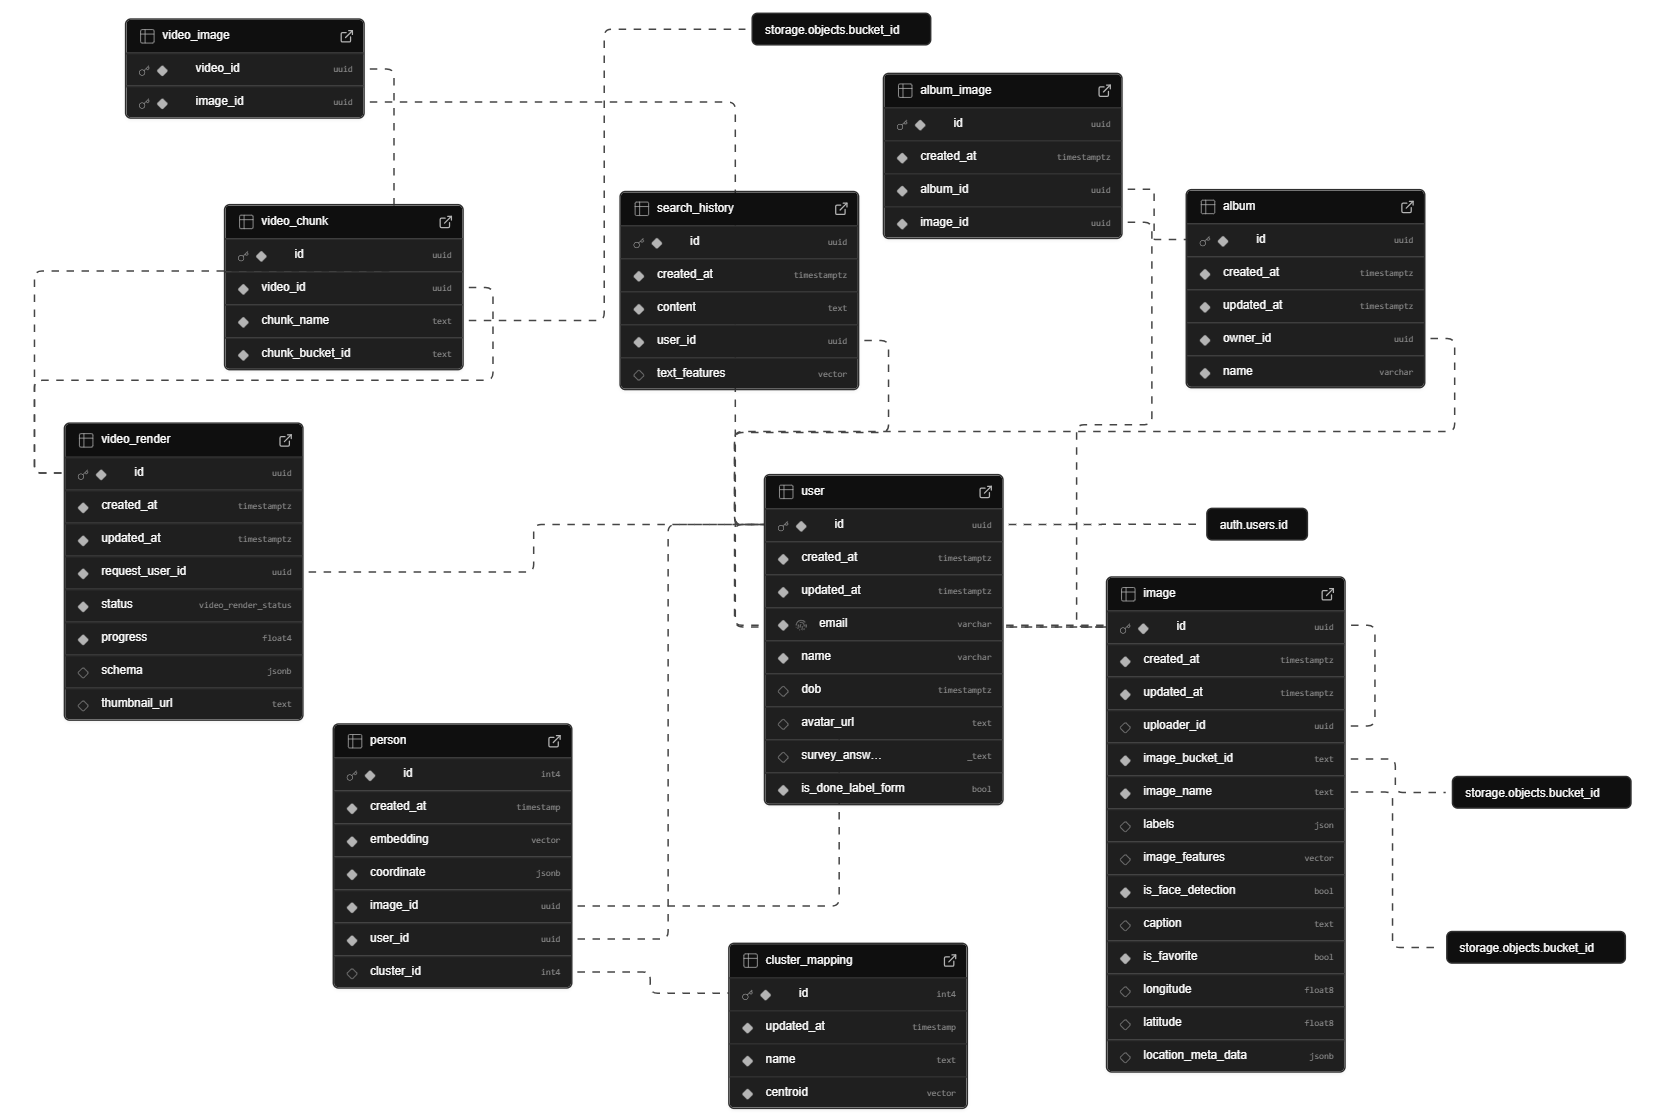
\includegraphics[width=1\textwidth]{figures/c3/3-4-database-graph.png}
    \caption{Cấu trúc cơ sở dữ liệu.}
    \label{fig:3-4-database-diagram}
\end{figure}